% 我记得还有个策略是 always connected 策略,因为之前,都是 发送完之后 直接deconnect的。。。
\section{M2M Related Energy Efficiency Studies}
\label{sec:overview-proposals}
To achieve energy efficiency at device side, the research community has done lots of efforts. In this section, we present, categorize and compare all found proposals related to energy issues for MTC in cellular networks. The energy issues may refer to energy saving, energy efficiency or power efficiency/saving. The result of classification and comparison among the proposals presented in this survey is resumed in Tab.~\ref{categorization-comparison}. 
\begin{table}[]
	\centering
	\caption{Categorization and comparison of energy/power saving-related proposals}
	\label{categorization-comparison}
	\resizebox{\textwidth}{!}{%
		\begin{tabular}{llllll}
			\hline
			Category                                                                                                           & Subcategory                                                                                   & Reference                                                                                                                       & Principle for energy saving                                                                                                                              & Drawback                                                                                                                                                                                     & Notes                                                                                                                                                         \\ \hline
			\multirow{3}{*}{\begin{tabular}[c]{@{}l@{}}Cooperative\\ design\end{tabular}}                                      & Clustering and relay                                                                          & \begin{tabular}[c]{@{}l@{}}\cite{kim2010snoop}\\ \cite{CYTu11}\\ \cite{YuanHo12}\\ \cite{azari14}\end{tabular}                  & \begin{tabular}[c]{@{}l@{}}Group devices into clusters;\\ Cluster head relays the messages for\\ other cluster member in the same\\ group\end{tabular}   & \begin{tabular}[c]{@{}l@{}}High energy consumption \\ for cluster head;\\ Scheduling and resource issues in\\ order to manage the interference;\\ Delay increase cause of relay\end{tabular} & \begin{tabular}[c]{@{}l@{}}It is possible to combine\\ cooperative relaying with\\ other emerging technologies\\ for the device-to-device\\ link\end{tabular} \\ \cline{2-6} 
			& \begin{tabular}[c]{@{}l@{}}Cooperation between MTC \\ server and MTC devices\end{tabular}     & \cite{Costa14}                                                                                                                  & \begin{tabular}[c]{@{}l@{}}Adjust MTC device setting\\ according to context\end{tabular}                                                                 & High complexity for MTC devices                                                                                                                                                              &                                                                                                                                                               \\ \cline{2-6} 
			& M2M gateway                                                                                   & \begin{tabular}[c]{@{}l@{}}\cite{ChenY10machine}\\ \cite{pereira2014towards}\\ \cite{ChenY09}\end{tabular}                      & \begin{tabular}[c]{@{}l@{}}Similar to clustering and\\ relay, except that M2M gateway\\ is a special network node\\ instead of a MTC device\end{tabular} & \begin{tabular}[c]{@{}l@{}}Installation and deployment \\ cost of M2M gateway\\ for operators\end{tabular}                                                                                   & \begin{tabular}[c]{@{}l@{}}Reduce implementation complexity \\ for MTC device.\\ \\ Possible to use LoRa gateway\\ as M2M gateway.\end{tabular}               \\ \hline
			\multirow{6}{*}{\begin{tabular}[c]{@{}l@{}}Design of \\ energy efficient\\ signaling and\\ operation\end{tabular}} & \begin{tabular}[c]{@{}l@{}}Modified DRX and \\ Idle state\end{tabular}                        & \begin{tabular}[c]{@{}l@{}}\cite{Gupta2013}\\ \cite{tirronen2012reducing}\end{tabular}                                          & \begin{tabular}[c]{@{}l@{}}Make MTC devices stay in low\\ power mode as long as possible\end{tabular}                                                    & High delay                                                                                                                                                                                   & \begin{tabular}[c]{@{}l@{}}Simple method to \\ achieve energy saving\end{tabular}                                                                             \\ \cline{2-6} 
			& Extending paging cycle                                                                        & \begin{tabular}[c]{@{}l@{}}\cite{3GPP/service-requirement}\\ \cite{3GPP/ranimprovements}\\ \cite{3GPP/TR/23887V12}\end{tabular} & \begin{tabular}[c]{@{}l@{}}Make MTC devices stay in low\\ power mode as long as possible\end{tabular}                                                    & High delay                                                                                                                                                                                   &                                                                                                                                                               \\ \cline{2-6} 
			& \begin{tabular}[c]{@{}l@{}}Reduction of RRC \\ Inactivity timer\end{tabular}                  & \cite{SCJha2013}                                                                                                                & \begin{tabular}[c]{@{}l@{}}Make MTC devices stay in low\\ power mode as long as possible\end{tabular}                                                    & Impact on H2H service                                                                                                                                                                        &                                                                                                                                                               \\ \cline{2-6} 
			& \begin{tabular}[c]{@{}l@{}}Group-based and \\ M2M- dedicated \\ paging mechanism\end{tabular} & \cite{ChaoCW11}                                                                                                                 & Group paging for MTC devices                                                                                                                             & \begin{tabular}[c]{@{}l@{}}May reduce the paging capacity\\ of H2H;\\ Scalability and bacward-\\ compatibility issues.\end{tabular}                                                          &                                                                                                                                                               \\ \cline{2-6} 
			& \begin{tabular}[c]{@{}l@{}}Removal \\ of unnecessary activities\end{tabular}                  & \cite{ChaoCW11}                                                                                                                 & \begin{tabular}[c]{@{}l@{}}Remove activities related to \\ mobility management (MM) \\ for MTC Device\end{tabular}                                       & \begin{tabular}[c]{@{}l@{}}Applicable uniquely for\\ M2M application with no \\ or low mobility\end{tabular}                                                                                 & \begin{tabular}[c]{@{}l@{}}Reduce the cost of MTC\\ device and energy\\ consumption\end{tabular}                                                              \\ \cline{2-6} 
			& \begin{tabular}[c]{@{}l@{}}Disconnect MTC-device \\ from network when inactive\end{tabular}   & \cite{scjha2014}                                                                                                                & \begin{tabular}[c]{@{}l@{}}Instead of staying in low power mode,\\ turn devices radio off\end{tabular}                                                   & High delay                                                                                                                                                                                   &                                                                                                                                                               \\ \hline
			\multirow{3}{*}{\begin{tabular}[c]{@{}l@{}}Radio resource\\ allocation\\ and packet\\ scheduling\end{tabular}}     & \begin{tabular}[c]{@{}l@{}}Formulation of\\ optimization problem\end{tabular}                 & \begin{tabular}[c]{@{}l@{}}\cite{AijazA13}\\ \cite{AijazTNCA14}\end{tabular}                                                    & \begin{tabular}[c]{@{}l@{}}Convert radio resource allocation\\ into an optimization problem with\\ constraints\end{tabular}                              & \begin{tabular}[c]{@{}l@{}}High complexity;\\ Scalability issues;\\ Possible impact for human\\ users.\end{tabular}                                                                          &                                                                                                                                                               \\ \cline{2-6} 
			& Optimized with periodicity                                                                    & \begin{tabular}[c]{@{}l@{}}\cite{Zhangy14}\\ \cite{GCMadueno14}\end{tabular}                                                    & Leverage the periodicity of MTC                                                                                                                          & \begin{tabular}[c]{@{}l@{}}Applicable uniquely to periodic\\ M2M applications;\\ Not easy applied in the presence\\ of different period values.\end{tabular}                                 &                                                                                                                                                               \\ \cline{2-6} 
			& Packet scheduling                                                                             & \begin{tabular}[c]{@{}l@{}}\cite{GotsisLA12}\\ \cite{SYLien11}\end{tabular}                                                     & \begin{tabular}[c]{@{}l@{}}Propose packet scheduling\\ adapted for cellular MTC context\end{tabular}                                                     & \begin{tabular}[c]{@{}l@{}}Compatibility with H2H;\\ May need modifications of the specification\end{tabular}                                                                                & Ensure QoS requirements                                                                                                                                       \\ \hline
			\multirow{3}{*}{\begin{tabular}[c]{@{}l@{}}Energy efficient \\ random access\\ and MAC\end{tabular}}               & New random access protocol                                                                    & \cite{laya14}                                                                                                                   & \begin{tabular}[c]{@{}l@{}}ALOHA-based random \\ access protocol is not \\ the best option for MTC\end{tabular}                                          & \begin{tabular}[c]{@{}l@{}}It may be difficult to find a specified\\ random access protocol suitable \\ for all cellular users\end{tabular}                                                  &                                                                                                                                                               \\ \cline{2-6} 
			& Fixed time alignment                                                                          & \cite{journals/icl/KoKBSKA12}                                                                                                   & Leverage the low mobility of MTC                                                                                                                         & \begin{tabular}[c]{@{}l@{}}Only applicable for M2M\\ with no mobility\end{tabular}                                                                                                           & Reduce the access collision                                                                                                                                   \\ \cline{2-6} 
			& \begin{tabular}[c]{@{}l@{}}Transmit message in \\ MAC PDU or preamble\end{tabular}            & \cite{ChenY10machine}                                                                                                           & \begin{tabular}[c]{@{}l@{}}Transmit message directly \\ in access reservation stage\end{tabular}                                                         & Scalability issues                                                                                                                                                                           & Reduce the signaling overhead                                                                                                                                 \\ \hline
		\end{tabular}%
	}
\end{table}


%%%%%%%%%%%%%%%%%%%%%%%%%%%%
\subsection{Cooperative Relaying}% 会不会有这样的误解:group-based 通信就是 群发呢?M2M gateway 算不算是 group-based communication呢?
Cooperative relaying, also called cooperative design~\cite{bartoli2011low}, can be interpreted as the process of devices helping each other to jointly achieve a goal more efficiently than each device could do on its own. The first possible form is group-based and relay (in fact, at most 2 hops) mechanism, which is very useful for energy saving, massive access control. A general and common description about group-based and relay transmission is illustrated in Fig.~\ref{fig:Illustration of M2M devices clustering}: all MTC devices are classified into several groups (some references call group as cluster). A certain device in each group is selected as coordinator (also can be called cluster header, group head) according to some criteria (e.g., QoS requirements~\cite{LienCL11}, link quality or location). The MTC devices other than coordinators transmit packets to their allocated coordinators, which relay the received packets to the BS (multiple-hop communication). In this model, there exist two links: MTCD-to-Coordinator (actually MTCD-to-MTCD link, since the coordinator is by nature still a MTC device) and Coordinator-to-BS. 
A basic issue is the interference between the two aforementioned links. This problem can be addressed by interference-based topology control algorithm~\cite{zhang2015interference}, specific scheduling, use of different frequencies between the two communications (but this is pricey in frequencies) or even using two different protocols as proposed in~\cite{YuanHo12}. In addition, how to enable and make the MTCD-to-MTCD link efficient is addressed by D2D communication~\cite{niu2015survey}\cite{niu2015exploiting}.
\begin{figure}[!t]
	\centering
	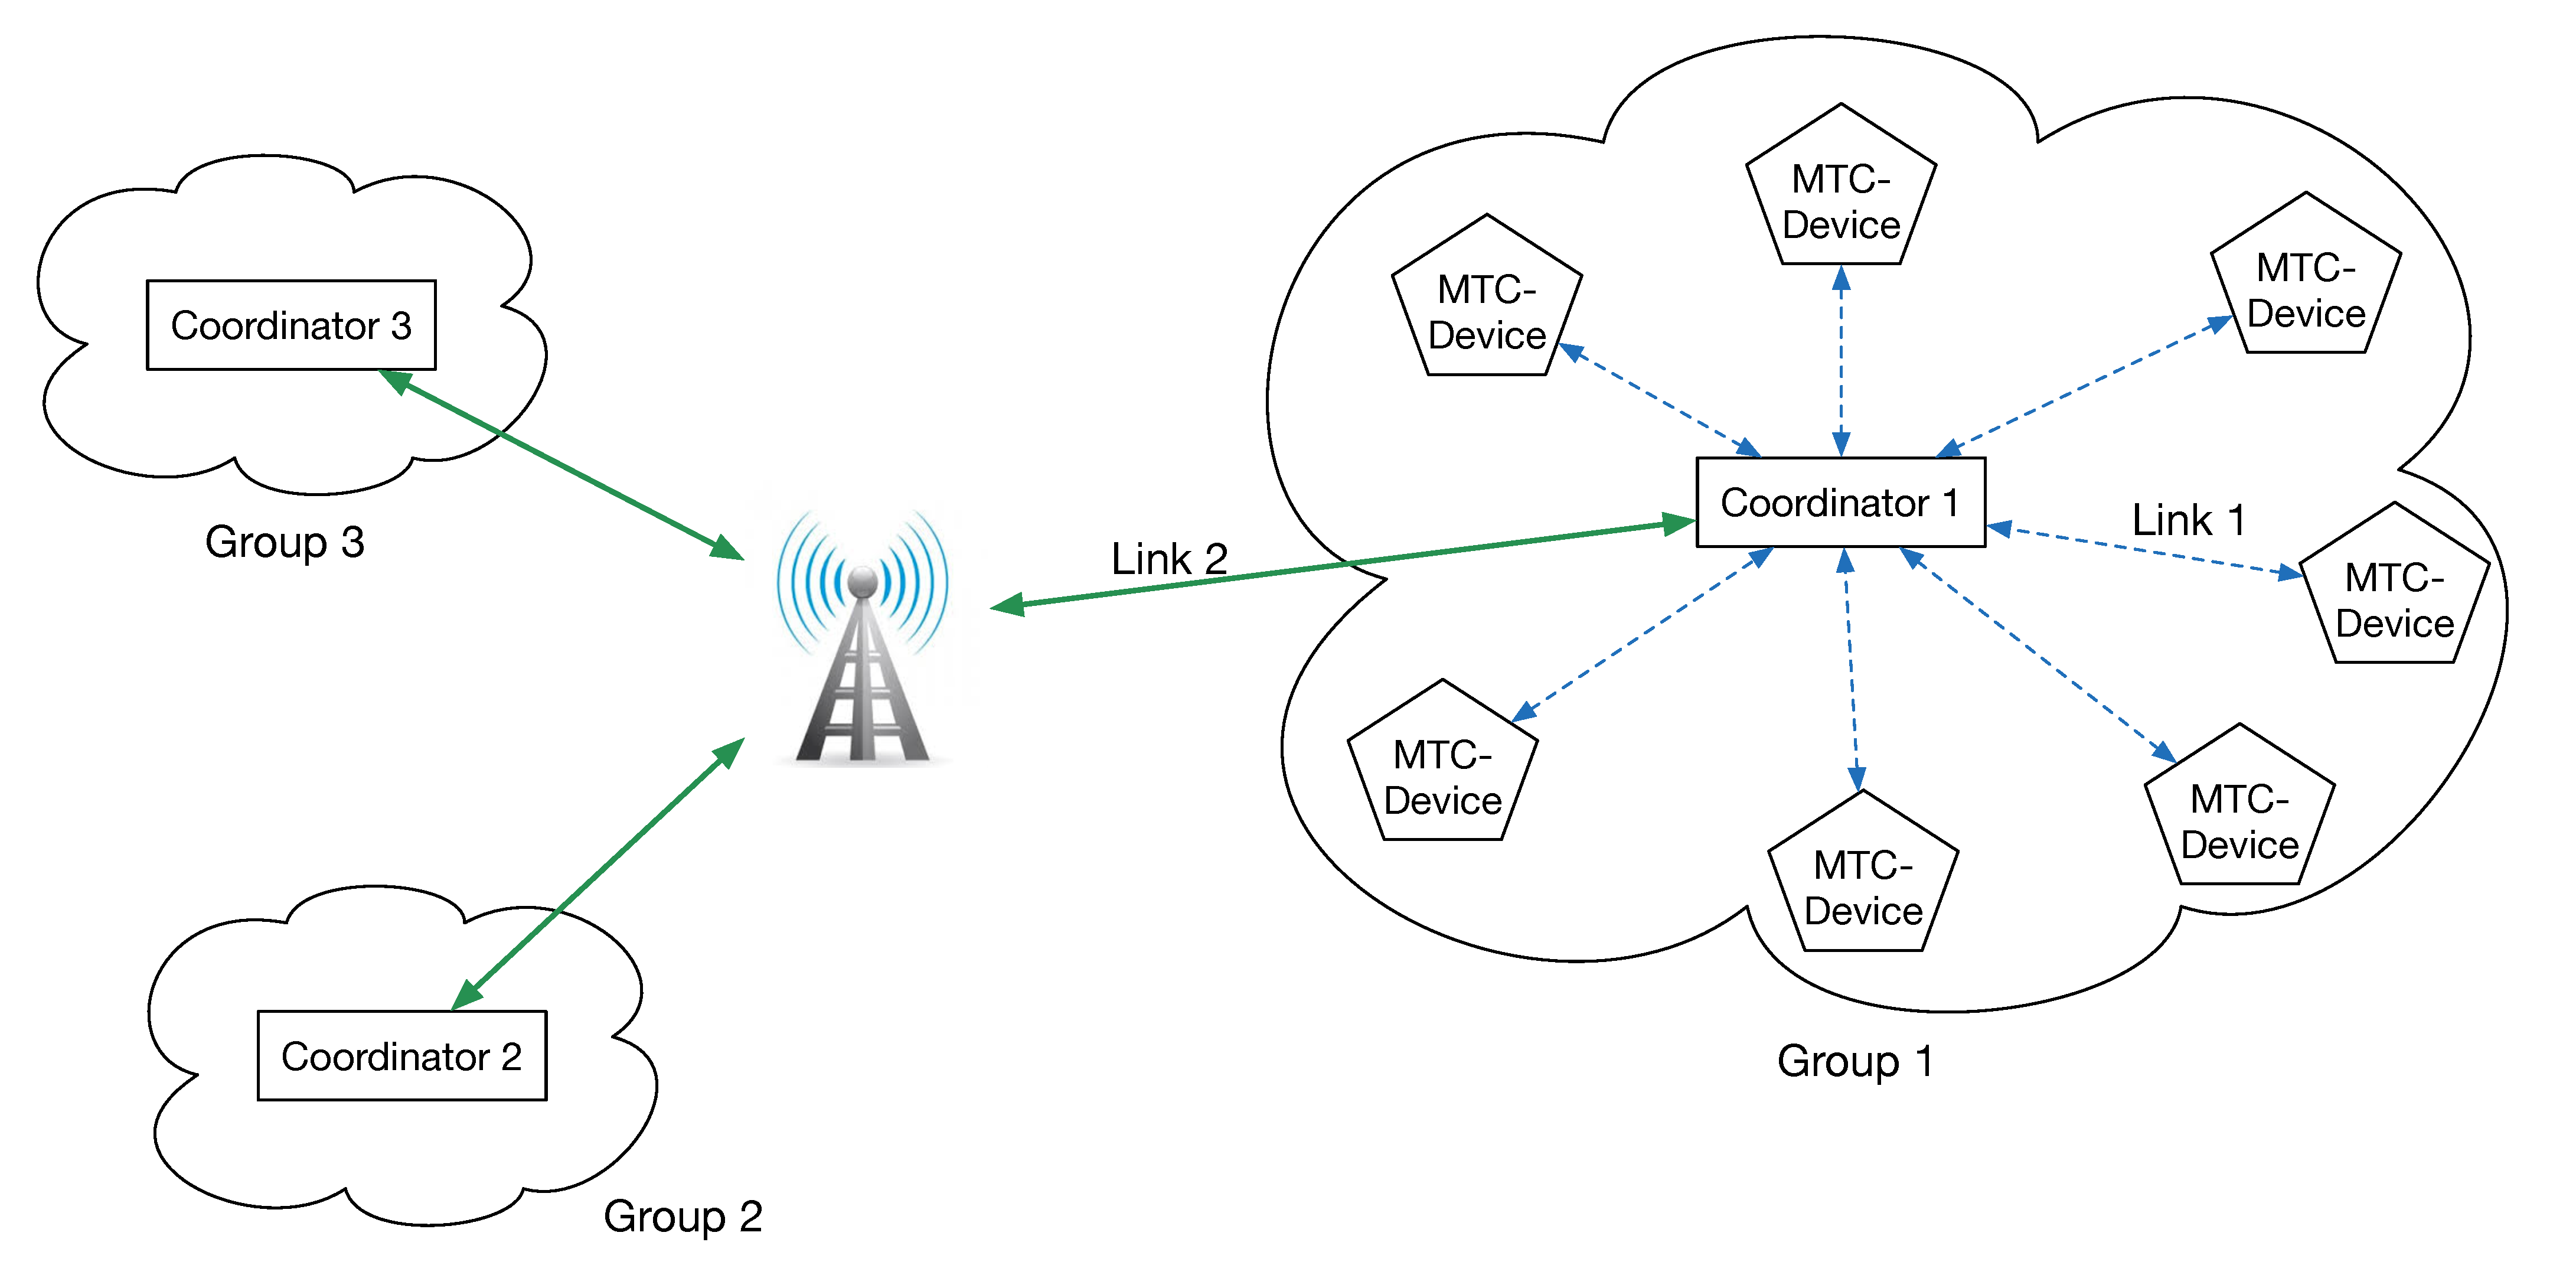
\includegraphics[width=0.8\linewidth,height=6cm]{Chapter2/Figures/Device_Clustering}
	\caption{Illustration of M2M devices clustering}
	\label{fig:Illustration of M2M devices clustering}
\end{figure}

The idea of group-based communication is presented in~\cite{kim2010snoop} but without clarifying grouping/clustering algorithms. In fact, the algorithms of device grouping and coordinator are a key factor influencing energy efficiency. A series of K-means (K-means clustering aims to partition $n$ observations into $k$ clusters in which each observation belongs to the cluster with the nearest mean) derived grouping and coordinator selection algorithms are proposed in~\cite{CYTu11}. Ho et al.~\cite{YuanHo12} propose a two-stage mechanism to minimize the energy consumption of all MTC devices. The first stage consist of MTC devices grouping, coordinator selection. The criteria for grouping and coordinator selection in each group are the minimization of energy consumption of this group. The second stage is that BS performs power allocation for each coordinator to further reduce energy consumption. However, it is difficult to obtain the closed-form solution for the formulated problem, the proposal of~\cite{YuanHo12} could achieve suboptimal result. 
An implementation of clustering and relay is presented in~\cite{azari14}: Intra-cluster communication uses CSMA/CA protocol with multiple-phases while resource reservation based protocol is used for communication between cluster head and BS. The drawback of the group-based and relay design relies in that:\begin{inparaenum}[(i)]
	\item although it is globally energy efficient for all the MTC devices, the cooperative relaying causes the cluster head to consume more energy than others;
	\item each MTC device should be equipped with multiple transceiver (e.g. OFDMA transceiver for Coordinator-to-BS link, TDMA transceiver for MTCD-to-Coordinator link), since every device is possible to be selected as coordinator.
\end{inparaenum}

The second form of cooperation is to introduce M2M gateway (may be called proxy~\cite{ChenY10machine}). The M2M gateway serves as an intermediary node to collect and process data for neighbor MTC devices. Thus, topologically, M2M gateway is very similar to the aforementioned cluster header, except that M2M gateway does not have its own data to transmit and may have a permanent energy source. 
It is preferred to use half-duplex M2M gateway to avoid self-interference and reduce implementation complexity~\cite{KanZheng12}.
The use of M2M gateway helps reduce the number of accessing devices, signaling overhead and contention thus helps improve energy efficiency. Chen et al.~\cite{ChenY10machine} give a simple work flow for MTC with M2M gateway. Pereira et al.~\cite{pereira2014towards} consider to use smartphones as M2M gateway between Base Station and MTC devices. The existing scheduled airliners used as relays between ground devices and satellites are presented in~\cite{plass2012concept}. It is also possible to add a gateway-like element node called M2M facilitator~\cite{ChenY09} between 3GPP RAN and Core Network, which is shown in Fig.~\ref{fig:M2M Facilitator}. 
M2M devices nominally communicate with M2M server. However, the M2M devices only communicate with base station and enter in sleep mode after the session with base station. Base station then transfers received data to M2M facilitator. Finally M2M facilitator is in charge of data transmission, retransmission and session termination with M2M server. Since the devices communicate only with M2M facilitator and the latter has no energy constraint, the protocol stack at device side can be significantly simplified to save energy consumption. The cost is that a fraction of protocol stack complexity is transferred to M2M facilitator. The inconvenient points of M2M gateway related proposals are:\begin{inparaenum}[(i)]
	\item operator should deploy M2M gateways to serve MTC devices, which may be of high cost;
	\item not flexible and dynamic compared with clustering-based group.
\end{inparaenum}
Compared with group-based and relay mechanism, the use of M2M gateway may be more energy efficient for devices. This is actually due to that a part of energy consumption of MTC devices is transferred to M2M gateway, which may have a permanent energy source.
\begin{figure}[!t]
	\centering
	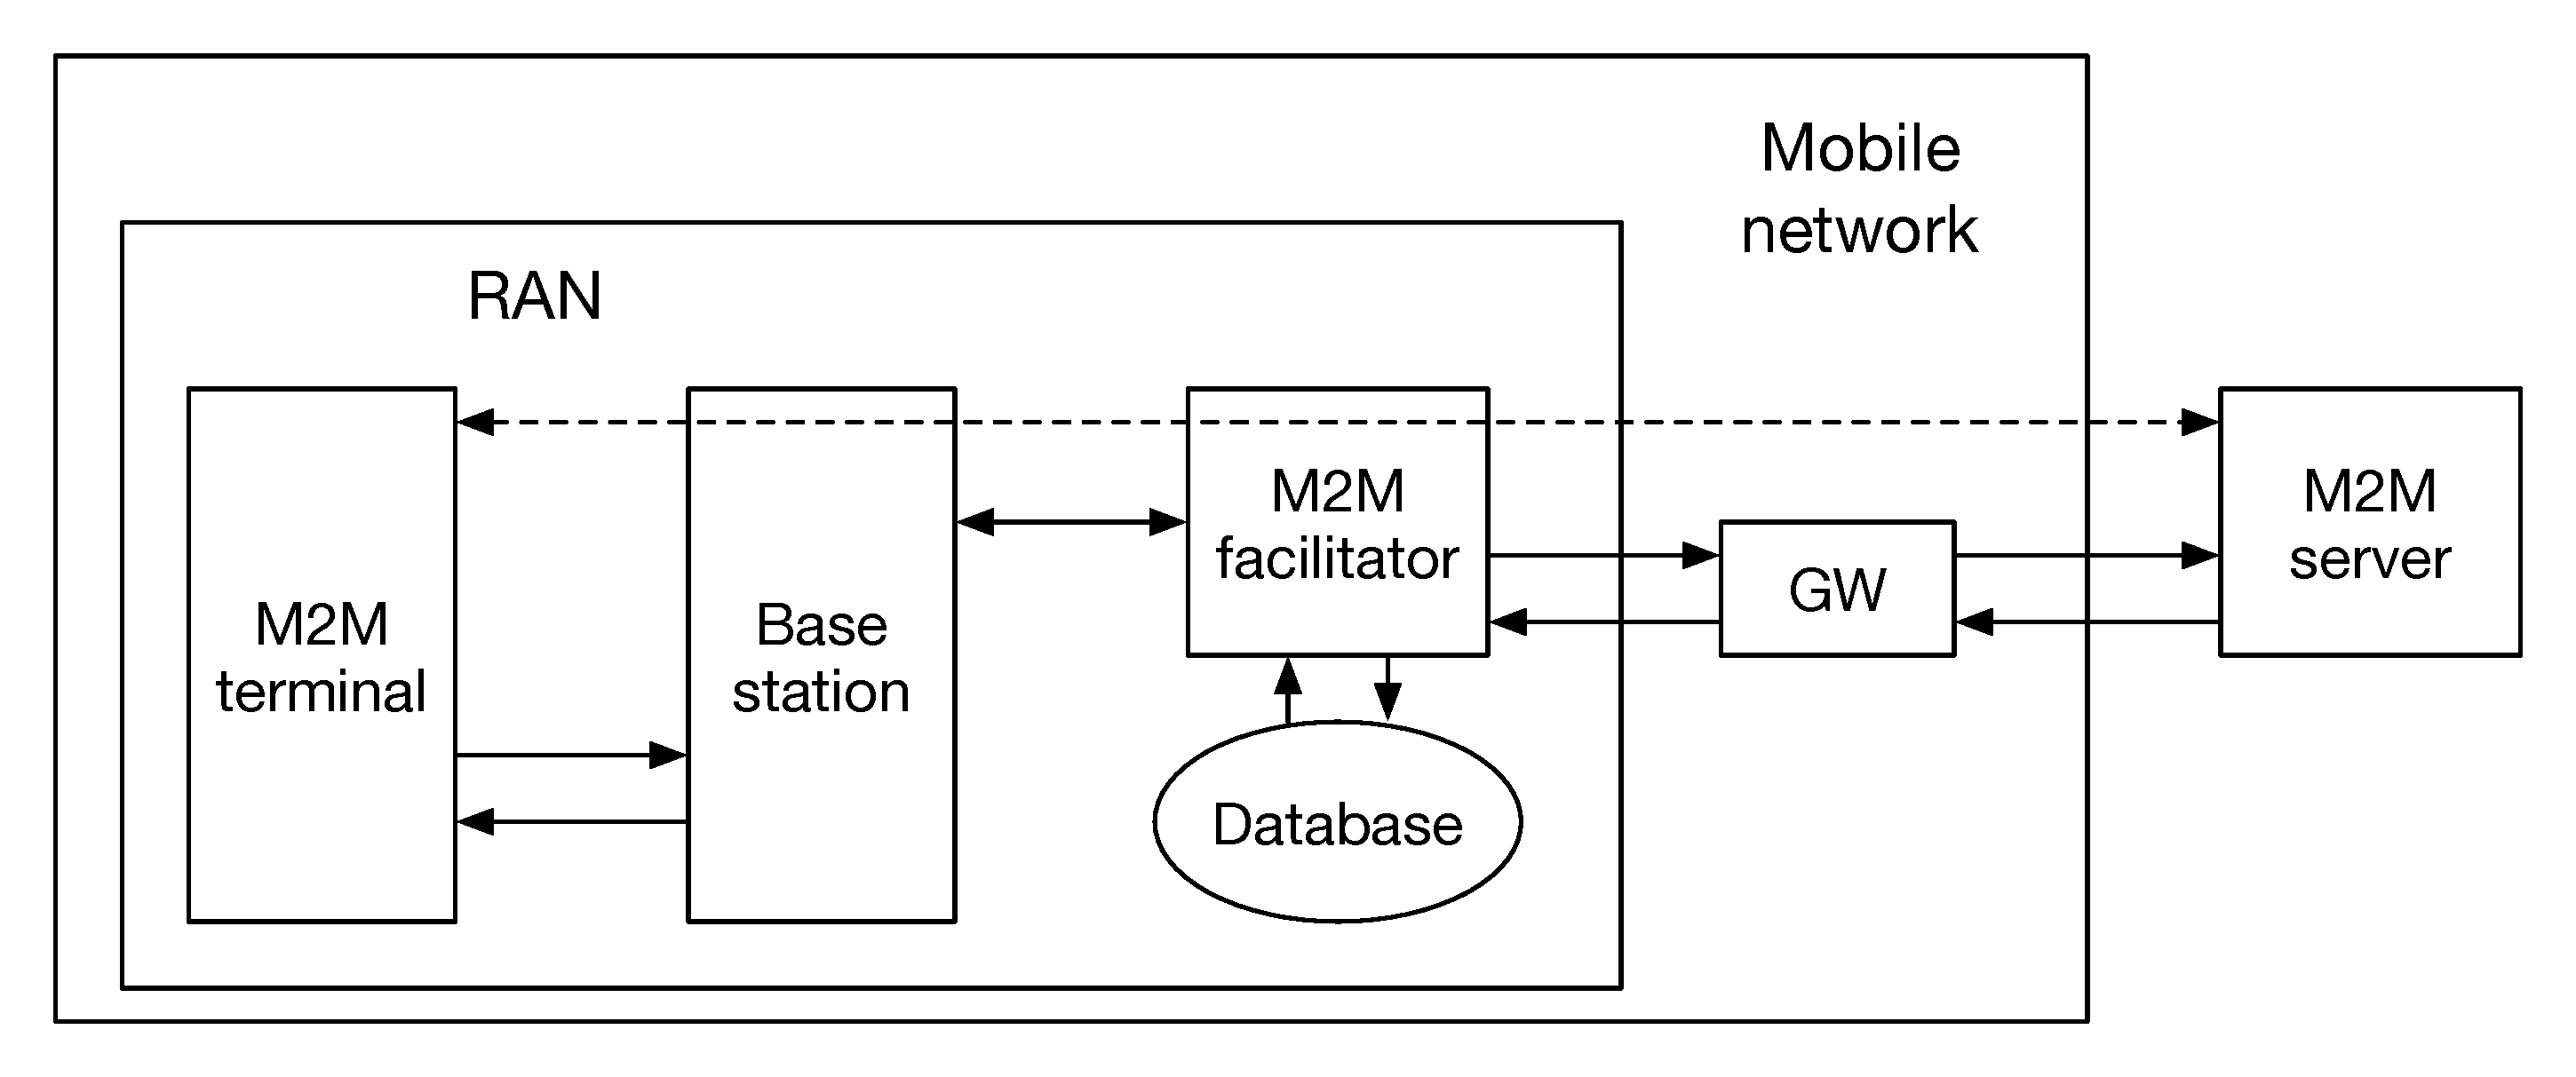
\includegraphics[width=0.9\linewidth]{Chapter2/Figures/M2M_Facilitator}
	\caption{Un-peer2peer cellular MTC architecture with M2M Facilitator. Source:~\cite{ChenY09} }
	\label{fig:M2M Facilitator}
\end{figure}

The third possible form of cooperation mechanism is context-based communication between MTC servers and MTC devices.  The philosophy of this axis is: intelligent algorithms can be deployed at application level to help M2M devices and overall network adjust their settings to improve energy efficiency. 
According to this philosophy the authors propose a context-aware framework based on context concept in~\cite{Costa14}. 
M2M devices send context-related information to MTC server, MTC server judges the data reporting mode(time-driven, query-driven, event-driven or hybrid) and QoS feature (real-time, priority and accuracy) then returns a set of output useful for setting device's behavior. 
This output involves inter-arrival time, average packet size, transmitting power, packet omission, etc. that could extend the operative lifetime of M2M devices.
%\subsection{Design of low-cost MTC-D}
\subsection{Design of energy efficient signaling and operation}
% 第一句话 说 H2H 的 UE 设计 是考虑 高速低延时的以及考虑了 mobility 的,但是对于MTC-D,这些不是追求的目标,所以需要重新设计 MTC-D的活动以及 节能机制。
An intuitive solution to achieve energy-efficiency for MTC is to design energy efficient signaling and simplify the operations leading to energy wasting. The key philosophy is to maximize the duration in low power state and reduce or even delete all operations unnecessary for MTC. The improvement possibilities are summarized as follows:\begin{inparaenum}[(1)]
	\\
	\item Adaption of DRX and Idle state: 3GPP has incorporated some energy/power saving mechanisms into their specification for H2H devices: for instance, Discontinuous Reception (DRX)~\cite{3GPP/ue-procedure-idle}. Due to long inter-arrival time between traffic sessions, MTC devices stay in LTE Idle states most time as it is designed as a low power state. In Idle state, MTC devices go to sleep to save battery and wake up periodically to inquire any system information (SI) update or downlink packet arrival via paging mechanism. However, the aforementioned mechanisms are still insufficient for MTC device, DRX and Idle state are adapted to improve device power saving in~\cite{Gupta2013}. The potential of trading high delay for reducing MTC devices battery consumption is studied in~\cite{tirronen2012reducing};\\ 
	\item Extending paging cycle: 3GPP considers to extend paging cycle for M2M devices~\cite{3GPP/service-requirement}\cite{3GPP/ranimprovements}\cite{3GPP/TR/23887V12}, but simulation results show that Extending Paging Cycle beyond $2.56$ seconds reduces the power consumption significantly for M2M traffic with small or medium values of inter-arrival time, but has no effect when the paging cycle is more than a limit~\cite{SCJha2013}. In addition, extension of Paging Cycle always increases the packet buffering delay;\\
	\item Reduction of RRC Inactivity timer: The network keeps MTC device in Connected mode even after the last packet delivery due to the RRC Inactivity timer in which MTC device still keep a high power, thus the impact of variation of RRC Inactivity Timer is explored and proved to be better than extending paging cycle~\cite{SCJha2013};\\
	\item Group-based and M2M-dedicated paging mechanism: To increase paging capacity multiple terminals are allocated with the same paging occasion (PO). H2H and M2M terminals may occupy the same certain paging occasion. If both are paged together, a large number of H2H terminals and MTC devices need to wake up at the same PO, which results in terminal power wasting. The solution to avoid this kind of power wasting is paging targets with group ID or device ID at dedicated paging occasion allocated uniquely for M2M devices~\cite{ChaoCW11};\\
	\item Removal of unnecessary operations: Even in Idle state, the MTC devices are not actually inactive: they are supposed to run activities related to mobility management (e.g., TAU procedure for LTE). Since MTC presents low mobility feature, it is possible to remove these unnecessary operations (Periodic AS measurement and NAS LAU/RAU/TAU procedure) for power saving~\cite{ChaoCW11};\\
	\item Disconnect MTC device from network when inactive: Since the device power consumption in Idle state is not negligible, it is possible to turn LTE radio off (i.e. disconnect the device from network) to obtain further power saving~\cite{scjha2014} and this is proved to be outperforming than approach of reducing RRC Inactivity timer. However, the gain of power saving is with cost of higher delay related to downlink packet. In addition, the network may also need to store the downlink data and the MTC device identities if the MTC device is off. 
\end{inparaenum}
\subsection{Radio resource allocation and packet scheduling strategies}
Radio resource allocation and packet scheduling strategies play a key role in the overall performance of OFDMA-based wireless networks~\cite{gotsis2007radio}. Most of research efforts in this field are about the downlink, which can for example improve network throughput and mitigate inter-cell interference~\cite{lopez2013distributed}\cite{ding2014small}. However, they have limited effectiveness about energy efficiency on MTC device side. In addition, MTC applications are usually uplink-centric, thus, it is import to design new radio resource allocation and packet scheduling schemes to achieve energy-efficiency.

Zheng et al.~\cite{KanZheng12} study the radio resource allocation scheme for the five possible links in M2M and H2H co-existence scenario: the eNB-to-UE link, the eNB-to-MTCD link, the eNB-to-MTCG link, the MTCG-to-MTCD link and the MTCD-to-MTCD link. They first design a new radio resource partition scheme and then propose efficient radio resource allocation algorithms in each partition to mitigate co-channel interference and enhance network efficiency, which is useful for energy-efficiency, but they just consider the data rate when allocating resource for both UE and MTC devices. 

Given that MTC usually features low data rate and emphasizes the delay requirement, Aijaz et al.~\cite{AijazA13} extend the work~\cite{KanZheng12} by formulating a bits-per-joule capacity maximization optimization problem. The resource constraint for UE is the minimum data rate and maximum tolerable packet delay for MTC devices. They propose two heuristic algorithms based on steepest descent approach to solve the optimization problem. Aijaz et al.~\cite{AijazTNCA14} further extend~\cite{AijazA13} by introducing the notion of statistical QoS (i.e., probability of exceeding a specific delay threshold) and solve the optimization problem with Canonical Duality Theory (CDT).

Radio resource allocation scheme can also leverage the periodicity of MTC, since a considerable of M2M users repetitively access to the networks to transmit collected data. Zhang et al.~\cite{Zhangy14} propose to use persistent resource allocation for periodic M2M applications and indicate the condition for multiplexing multiple MTC devices with different reporting periods. Madueno et al.~\cite{GCMadueno14} propose a periodically occurring pool of resources that are reserved for M2M communications and shared for uplink transmission by all MTC devices. Song et al.~\cite{qipeng2015an} propose a multiple-period polling service in LTE transport network to avoid random access procedure by leveraging the periodicity feature of M2M.

Group-based feature can be leveraged when designing M2M-compatible radio resource allocation strategies. Since MTC devices in the same cluster are assumed to have exactly the same QoS requirements, a grouping-based radio resource allocation algorithm~\cite{SYLien11}\cite{LienCL11} is proposed for LTE-A base stations according to packet arrival rate and maximum jitter. The access grant time interval (AGTI) is periodically allocated for each MTC device cluster according to cluster priority. All the MTC devices of a same cluster occupy an equal number of Resource Block (RB) in allocated AGTI. The shortcomings of this proposal are:\begin{inparaenum}[i)]
	\item the number of served MTC devices is limited due to the inefficient utilization of resource;
	\item the base station only supports a unique packet size for all MTC devices;
	\item the proposal is not scalable since BS has to know in advance how many clusters in its coverage;
	\item the supported QoS classes are limited.
\end{inparaenum} 

Since the packet delay employed in~\cite{SYLien11} is a deterministic bound, Gotsis et al.~\cite{GotsisLA12} extend work of~\cite{SYLien11} by using a statistical QoS (also used in~\cite{AijazA13}), which refers to the probability of exceeding a specific delay threshold. They propose an analytical model to study the performance of period scheduling algorithm in terms of statistical QoS metric with modeling the arrival traffic as Poisson process. They also enhance the periodic scheduling in~\cite{SYLien11} with queue-awareness in which devices with larger queues than others are first granted access to the scheduled AGTI with an extra cost in complexity and signaling. 

To overcome the issue of QoS classes, two uplink packet scheduling strategies are proposed in~\cite{lioumpas2011uplink}, which take into account both the channel conditions and the maximum allowed delay of each device, however, it suffers from increased signaling requirements and is just able to serve limited number of MTC devices. In~\cite{YuanHo12} a resource allocation scheme (i.e., optimal transmit power allocation over RBs) for M2M traffic over OFDMA frames is proposed, assuming a two-hop access to the LTE network though a coordinator. This work achieves the reduction of energy consumption, but does not take into account QoS issue of MTC such as the delay requirements.
%以下一段介绍来自\cite{lioumpas2011uplink}
%The scheduler in LTE has a central role, which is to determine which RBs will be occupied by each user every TTI, according to specific rules, which usually exploit the time and frequency channel variations at the users' RBs. In current LTE systems, schedules are mostly designed for maximizing the overall throughput, while taking into account some fairness and QoS rules. Because of the limited number of different service (i.e. voice, video and web) and the relatively small difference in their delay tolerance constraints (i.e. ranging from $100$ to $500$ ms), the channel quality of each RB is the major factor that characterizes most LTE scheduling algorithms. In M2M communications, the large number of devices and the vast diversity of applications creates a totally different landscape, where channel quality and QoS constraints are equally important for the scheduling algorithms. For example, the large number of devices is expected to frequently lead to situations where the number of requests will be larger than the maximum number of RBs. In such situations, it is important to know which devices can tolerate a denial of service and for how long. Moreover, in M2M communications, exploiting the QoS requirements of the devices for energy saving, is particular crucial.
%In the literature \cite{Zanella13}, the authors considered the challenges and potential solutions for providing cellular-based massive access of battery-constrained devices in a wide-area, as envisioned by the emerging paradigms of smart cities and the Internet of Things. The challenge builds upon the premise that: 1) there is no consolidated understanding of the limits on control signaling and PHY/MAC overhead for supporting massive access, short data packets, and extremely variable transmission patterns; and 2) there exist no technical solutions that maximize the amount of users to be served under extremely severe constraints on battery capacity and transceiver complexity. They have provided a first insight into those limits and solutions and illustrated some new PHY, MAC, and architecture solutions with the purpose of serving many devices with short and correlated packets, and limited battery life. They exploit inherent characteristics of M2M signals to reduce the signaling overhead and make MTD data transmission more cost and energy-effective.
\subsection{Energy-efficient random access procedure and MAC}
The currently standardized random access procedure, for example, in LTE networks, is designed and optimized for large amount of data transmission and limited UEs, thus it suffers from random access overload issue which leads to high collision probability and waste of energy. The improvement works about random access procedure have been attracting the attention of research community. Current random access optimization research efforts can be resumed into two categories:\begin{inparaenum}[i)]
	\item improvement for currently employed ALOHA-like random access procedure;
	\item designs of non-ALOHA procedure.
\end{inparaenum}

For the first category, the focus is to reduce either signaling overhead for small data transmission or contention probability, since both reduce the transmitted bits for MTC devices thus help energy saving. For MTC with lots of fixed location machines, Ko et al.~\cite{journals/icl/KoKBSKA12} propose a novel random access scheme based on fixed TA (timing alignment) for OFDMA-based cellular system. The proposal is based on the assumption that the TA value between each fixed location machine device and eNB is fixed and unchanged, the MTC devices store the TA value acquired from the initial RA access and compare it with the TA values obtained from the subsequent random access procedure. In case of mismatch of TA values,  MTC devices directly start retransmission procedure to avoid possible collision after waiting a randomly selected backoff time. Otherwise, the devices continue the conventional procedure. However, this proposal is only applicable to M2M with stationary devices and has limited effect on energy-efficiency. 

For M2M applications with small data transmission, establishing RRC connection, network connection to transmit several bits is deemed as wasteful. Thus, Chen et al. \cite{ChenY10machine} suggest either \begin{inparaenum}[i)]
	\item use the MAC PDU that should carry the RRC signaling to carry the data;
	\item define special preamble to transmit coded data.
\end{inparaenum}
The drawbacks of \cite{ChenY10machine} are:\begin{inparaenum}[i)]
	\item the solution based on the preambles is not very scalable due to the limited amount of available preambles;
	\item for a long term view, the transmission of data in control plane violate the principle of separation between control plane and data plane. 
\end{inparaenum} 
Wiriaatmadja et al.~\cite{wiriaatmadja2015hybrid} propose to simplify the data communication procedure by allowing MTC devices to send data right after preamble transmission without explicitly establishing a connection.

For the congestion in random access, Physical Downlink Shared Channel (PDSCH) resources of LTE are deemed sufficient in most communication scenarios. To ease the congestion on the air interface, those downlink assignments and uplink grants for MTC devices, which cannot be served by Physical Downlink Control Channel (PDCCH), can be aggregated into a transport block on PDSCH identified by a special  Radio Network Terminal Identifier (RNTI) called MTC-RNTI~\cite{transaction/yang13}. MTC devices monitor PDCCH channel with their own cell RNTI and MTC-RNTI simultaneously. Game theory has been used for the context of cellular M2M to optimize preamble allocation \cite{MHasan13}. In addition, a detailed random access related proposals are summarized in~\cite{laya14}, which can be a complement of our categorization.

Random access protocols can be categorized into two families: ALOHA family and tree family~\cite{WXu92}. Andres et al.~\cite{laya14} claim that ALOHA based RACH procedure is not suitable for MTC. Instead they mention that  RACH procedure based on distributed queuing (DQ) is more promising. The concept of DQ~\cite{WXu92} was proposed twenty years ago and then demonstrated in other literatures in terms of stability and near optimum behavior. DQ is based on the combination of a m-array tree splitting algorithm with a smart set of simple rules that allow organizing every device in one out of two virtual queues. Due to the rules of DQ, it behaves as a random access method for low traffic loads, and it switches smoothly and seamlessly to a reservation access method as the traffic load increases. The authors conduct some ongoing research efforts applying DQ ideas within LTE/LTE-A systems. Dhillon et al. \cite{Dhi13} suggest to implement a load dependent access scheme wherein uncoordinated strategy for light load and coordinated strategy for heavy load. Bontu et al.~\cite{bontu2014wireless} propose a new UL physical, transport and logical channel: Common Traffic Channel (CTCH), UL simultaneous-access shared channel (UL-SSCH) and physical uplink simultaneous access shared channel (PUSSCH). Aforementioned channels enable M2M devices to simultaneously transmit data packet in the same radio resource. They also propose to transmit control signaling through in-band transmission in the user plane control.
%\input{TAB-proposals-resume.tex}

In addition, there also exist mathematical works that are not categorized into Tab.~\ref{categorization-comparison}, but they provide useful design guidelines to help improve device side energy efficiency. For example, in~\cite{khoshkholgh2015modeling}, the transmission energy is modeled as a function of transmission power, packet size and link capacity.  A cumulative distribution function (CDF) of energy consumption for large-scale MTC is derived by using stochastic geometry. In~\cite{Dhi13}, the comparison in terms of energy and power efficiency between uncoordinated and coordinated multiple access strategies are conducted. In ~\cite{song2016evaluation}, the work~\cite{Dhi13} is extended by considering various packet size and imperfect power control.
%Reviewers think that the comparison among all aforementioned researches are suggested to be more rich...

In fact, the cellular networks evolution trend is always to seek for a trade off between diverse performance metrics such as energy efficiency, packet delay, user data rate, etc. Hence, the gain of energy efficiency is inevitably with cost of a certain degradation of other performance metrics. For example, the cooperative relaying achieves energy efficiency with more packet delay due to multiple-hop transmission. The design of energy efficient signaling and operation, such as disconnection MTC devices from network when inactive, surely saves energy consumption but introduce higher delay for downlink packet, and the effort in this direction is not systematic. The energy efficient uplink radio resource allocation and packet scheduling schemes provide a systematic manner to gain energy efficiency for MTC, but they may lead to either serving less number of MTC devices and supporting limited QoS classes or bringing more signaling messages in radio access networks. More importantly, it is difficult to design schemes simultaneously satisfying the QoS provisioning for both human and MTC users. The random access can be designed to reduce the retransmission probability for MTC users, but human users may suffer from degradation of service, due to the limited radio access resources. Therefore, it is very important to jointly apply the aforementioned approaches to gain device side energy efficiency and seek for a trade off with other system performance. For example, the random access procedure can be optimized by applying cooperative relaying to reduce the direct links towards the base station. The energy efficient uplink radio resource allocation algorithms can be jointly designed with random access procedure: allocate more resources for PRACH in case of overload or limit the number of access devices when no radio resource for data transmission, etc.

%jointly considering the net- work capacity, energy consumption, and adequate QoS.